\section{Техническое задание}
\subsection{Основание для разработки}

Полное наименование системы: \quotes{Интерпретатор функционального языка программирования с поддержкой метапрограммирования}.

Основанием для разработки программы является приказ ректора ЮЗГУ от «15» апреля 2024 г. №1779-с «Об утверждении тем выпускных квалификационных работ».

\subsection{Цель и назначение разработки}

Цель этой работы -- разработка программной системы, позволяющей сокращение размера исходного кода программ за счёт метапрограммирования.

Для достижения этой цели было принято решение разработать интерпретатор функционального языка программирования с поддержкой метапрограммирования. Основной задачей разработки является разработка программного обеспечения, способного анализировать и исполнять программы, написанные на функциональном языке программирования, а также обеспечивать возможности генерации и изменения кода на этом языке с использованием инструментов метапрограммирования.

Интерпретатор, созданный в рамках данной работы, должен иметь все ключевые функции, обеспечивающие поддержку парадигм метапрограммирования и функционального программирования. Для их реализации будет разработан простой и минималистичный функциональный язык программирования, называемый \quotes{демонстрационный язык программирования} (ДЯП), поддерживающий метапрограммирование.

Таким образом, интерпретатор сможет работать с  числами, строками, переменными, функциями, лямбда-выражениями, макросами и другими необходимыми конструкциями, обеспечивающими разработчику возможность использовать метапрограммирование для создания адаптивных и реплицируемых приложений.

Задачами данной разработки являются:
\begin{itemize}
\item разработка синтаксиса ДЯП, достаточного для реализации функционального программирования и метапрограммирования;
\item разработка объектов, используемых для представления интерпретируемого исходного кода внутри интерпретатора;
\item разработка сборщика мусора;
\item разработка лексического анализатора для созданного языка;
\item разработка синтаксического анализатор для созданного языка;
\item разработка исполнителя инструкций;
\item реализация примитивных функций созданного языка.
\end{itemize}


\subsection{Описание разрабатываемого языка}

Разрабатываемый язык является подмножеством языка программирования \quotes{Common Lisp} и сосредотачивается на реализации его базовых возможностей по работе с данными и метапрограммирования. Потому, он будет иметь функциональность для работы с переменными, функциями, лямбда-выражениями, функциями высшего порядка, числами, строками, символами, списками и массивами. Введутся базовые функции для обработки данных, включая операции сложения чисел, выделения подстрок из строк, определения имени символа по символьному объекту и другие, реализующие минимально необходимые возможности для манипуляции данными. Также будет включена система макросов как основной элемент реализации метапрограммирования.

\subsubsection{Алфавит языка}
Алфавит языка программирования -- это перечень символов, допустимых к использованию для записи синтаксических конструкций этого языка \cite{e4}. Символом может быть как буква, цифра или знак препинания, так и любой другой знак, рассматриваемый как неделимый элемент языка.

Алфавит разработанного языка включает:
\begin{itemize}
	\item латинские символы верхнего и нижнего регистра;
	\item римские цифры;
	\item символы, зарезервированные под описание конструкций языка, перечисленные через пробел: ' ` , . '' \#;
	\item другие символы, перечисленные через пробел: + - * / = \_ \& | < >.
\end{itemize}

\subsubsection{Лексемы, распознаваемые лексическим анализатором}

Список наименований лексем, распознаваемых лексическим анализатором, а также их символьное представление или пример:
\begin{itemize}
	\item десятичное и шестнадцатеричное целое число: 10, 0xFFAA;
	\item вещественное число: 1.34;
	\item символ: A;
	\item цитата: ';
	\item квазицитата: `;
	\item запятая: ,;
	\item запятая-at: ,@;
	\item решётка: \#;
	\item левая скобка: (;
	\item правая скобка: );
	\item точка: .;
	\item строка: \quotes{a b c v ddd};
	\item неизвестный объект -- объект, который ЛА не смог определить;
	\item конец потока.
\end{itemize}

Помимо этого, для удобства разработчика, синтаксисом языка предусмотрена возможность добавлять в код комментарии. Комментарий начинается со знака ‭\quotes{;} и заканчивается переносом строки.

Символ \quotes{\textbackslash} используется для экранирования.


\subsubsection{Типы данных}
Для языка программирования были определены шесть фактических типов данных и два псевдотипа:
\begin{itemize}
	\item Число -- десятичные и шестнадцатеричные числа, размер которых ограничен 28 битами (от -134217728 до 134217727). Например: 10, 0xFFAA;
	
	\item Большое число -- число, для хранения которого необходимо более 28 бит. Например: 134217728;
	
	\item Строка -- произвольный набор алфавитных символов, задающийся в двойных кавычках. Например: \quotes{ab 12 /};
	
	\item Символ -- именованный нечувствительно к регистру объект, который может указывать на некоторое значение -- число, лямбда-выражение, макрос, строку, массив, список или функцию. Имя символа должно начинаться с буквы или разрешенного символа и может содержать буквы, цифры, символы. Таким образом, переменные, функции и другие объекты языка, к которым можно обращаться по имени, являются символами, содержащими указатель на объект с данными, заданными для этого символа. Пример символа: A;
	
	\item Атом -- псевдотип, специальное название для обозначения примитивных объектов данных, которые не разбиваются составляющие: символы, числа и строки;
	
	\item Точечная пара -- это хранилище, содержащее только два элемента, называемые левым и правым. Пара носит название точечной, так как в синтаксисе эта конструкция представляет собой два элемента, разделённые точкой, обрамлённые в круглые скобки. Например: ('a . 2);
	
	\item Список -- хранилище с последовательным доступом к элементам, содержащее ноль или более атомов, разделенных пустотами (пробелы или переводы строк) и заключённых в круглые скобки. С точки зрения внутреннего представления списки являются синтаксическим упрощением, реализованным за счёт точечных пар, где левый элемент пары -- значение, а правый -- указатель на следующую точечную пару. Таким образом выстраивается цепь точечных пар. Правый элемент последнего элемента такой цепи указывает на специальное значение nil. Списки могут содержать в себе другие списки. Пример: (x 2 'p);
	
	\item Массив -- хранилище с прямым доступом к элементам (можно обращаться по индексу), содержащее ноль или более атомов, разделенных пустотами и заключённых в круглые скобки, перед открывающей ставится \#. Массивы могут содержать в себе другие массивы. Пример: \#(3 6 9).
\end{itemize}

Для идентификации типов в интерпретаторе будет использоваться перечисление, содержащее следующие значения:
\begin{itemize}
	\item NUMBER: число;
	\item BIGNUMBER: большое число;
	\item SYMBOL: символ;
	\item PAIR: точечная пара (список);
	\item STRING: строка;
	\item ARRAY: массив.
\end{itemize}

S-выражение -- это основной элемент синтаксиса языка, который может быть атомом или списком. S-выражения нечувствительны к регистру. Все инструкции в ДЯП являются s-выражениями, из чего следует, что программный код представляет собой множество s-выражений \cite{e10}.

Для обозначения \quotes{истинного} и \quotes{ложного} используются зарезервированные объекты-символы \quotes{T} и \quotes{NIL} соответственно.

\subsubsection{Функции и лямбда-выражения}

В языке программировании применяются функции и лямбда-выражения.

Функция представлена в виде списка, содержащего символ, имя которого соответствует имени функции, список аргументов и тело функции.

Для объявления новой функции используется функция defun, имеющая следующий синтаксис:
(defun name (p \textsubscript 1 ... p \textsubscript n) e), где name -- имя объявляемой функции, p \textsubscript 1 ... p \textsubscript n -- параметры функции, e -- тело функции.

Вызов функции -- список, где первый элемент это имя функции, а последующие являются её аргументами.

Синтаксис вызова функции:
(name a \textsubscript 1 ... a \textsubscript n), где name -- имя вызываемой функции, а a \textsubscript 1 ... a \textsubscript n -- передаваемые функции аргументы.

Лямбда-выражения объявляются идентично функциям, но вместо функции defun используется lambda и, так как лямбда-выражения безымянны, имя не задаётся.

Для вызова лямбда-выражения необходимо создать список, где первым элементом будет само лямбда-выражение, а a \textsubscript 1 ... a \textsubscript n -- передаваемые выражению аргументы: 
((lambda (p \textsubscript 1 ... p \textsubscript n) e) a \textsubscript 1 ... a \textsubscript n).

При вызове, сначала вычисляются все аргументы a \textsubscript 1 ... a \textsubscript n. Затем каждому параметру p \textsubscript 1 ... p \textsubscript n ставится в соответствие вычисленное значение аргументов a \textsubscript 1 ... a \textsubscript n. После этого вычисляется выражение e, содержащее параметры, вместо которых будут подставлены их значения.

Например:

< ((lambda (x y) (cons x (cdr y))) 'z '(a b c))

> (Z B C).

Это лямбда-выражение с помощью функции cons создаёт список, состоящий из значения аргумента x и обрезанного со второго элемента с помощью cdr списка y. Результатом выполнения этого кода будет новый список -- \quotes{(Z B C)}.

Функции и лямбда-выражения могут быть получены и переданы в качестве аргументов или возвращены из функции и лямбда-выражения, как и необходимо в функциональной парадигме программирования.


\subsubsection{Макросы}

В ДЯП для создания макросов применяется функция defmacro, а также операторы quote, backquote и comma.

Функция defmacro имеет следующий синтаксис:
(defmacro name (a \textsubscript 1 ... a \textsubscript n) e), где name -- имя макроса, a \textsubscript 1 ... a \textsubscript n -- параметры макроса, e -- тело макроса.

Пример использования:

\begin{enumerate}
	\item Создам макрос, задающий шаблон для генерации выражения:
	
	(defmacro test (var val) (list 'defvar var val)).
	
	При вычислении этот макрос заменится списком, первым элементом которого будет символ defvar для объявления переменной, а последующими -- переданные при вызове макроса аргументы:
	
	(defvar var val).
	
	Для того, чтобы посмотреть что собой будет представлять вычисленный макрос с переданными ему аргументами, имеется функция \quotes{macroexpand}, куда вызов макроса передаётся в виде списка, на который применено цитирование:
	
	< (macroexpand '(test a 2))
	
	> (defvar a 2).
	
	\item Вызову макрос с символом \quotes{abc} и числом 100 в качестве аргумента. При вызове происходит вычисление тела макроса (развертывание макроса):
	
	\quotes{(test abc 100)} преобразуется в \quotes{(defvar abc 100)}.
	
	\item Получившееся выражение вычисляется. Список расценивается как код, который определяет переменную и присваивает ей значение:
	
	(defvar abc 100).
\end{enumerate}

По итогу был создан макрос test, объявляющий переменную с именем, переданным ему в качестве первого аргумента, и значением в качестве второго.

Кавычки (') -- символ, используемый для реализации цитирования -- предотвращения вычисления выражения. Например, выражение (* 2 2) будет автоматически вычислено и даст 4, в то время как '(* 2 2) будет восприниматься как список символов.

Но для предоставления по-настоящему широкого спектра возможностей для разработчика, необходимо реализовать инструментарий, позволяющий выполнять частичные вычисления -- квазицитирование.

Для того будут использоваться символы обратной кавычки \quotes{`} и запятой \quotes{,}. Обратная кавычка будет указывать на то, что выражение содержит вычисляемые элементы, а запятая укажет на них. Кавычка, обратная кавычка и запятая действуют на вычисление только того выражения, перед которым стоят.

Пример использования:

< (defvar b 12) (print `(+ a ,b))

> (+ A 12).

Таким образом, \quotes{+} и \quotes{a} были восприняты интерпретатором как символы и остались невычисленными, а \quotes{b} заменён значением соответствующей переменной.

\subsection{Компоненты интерпретатора}

На рисунке \ref{kompdiagram:image} в виде UML-диаграммы показаны компоненты, составляющие интерпретатор \cite{e26}.

\begin{figure}[ht]
	\center{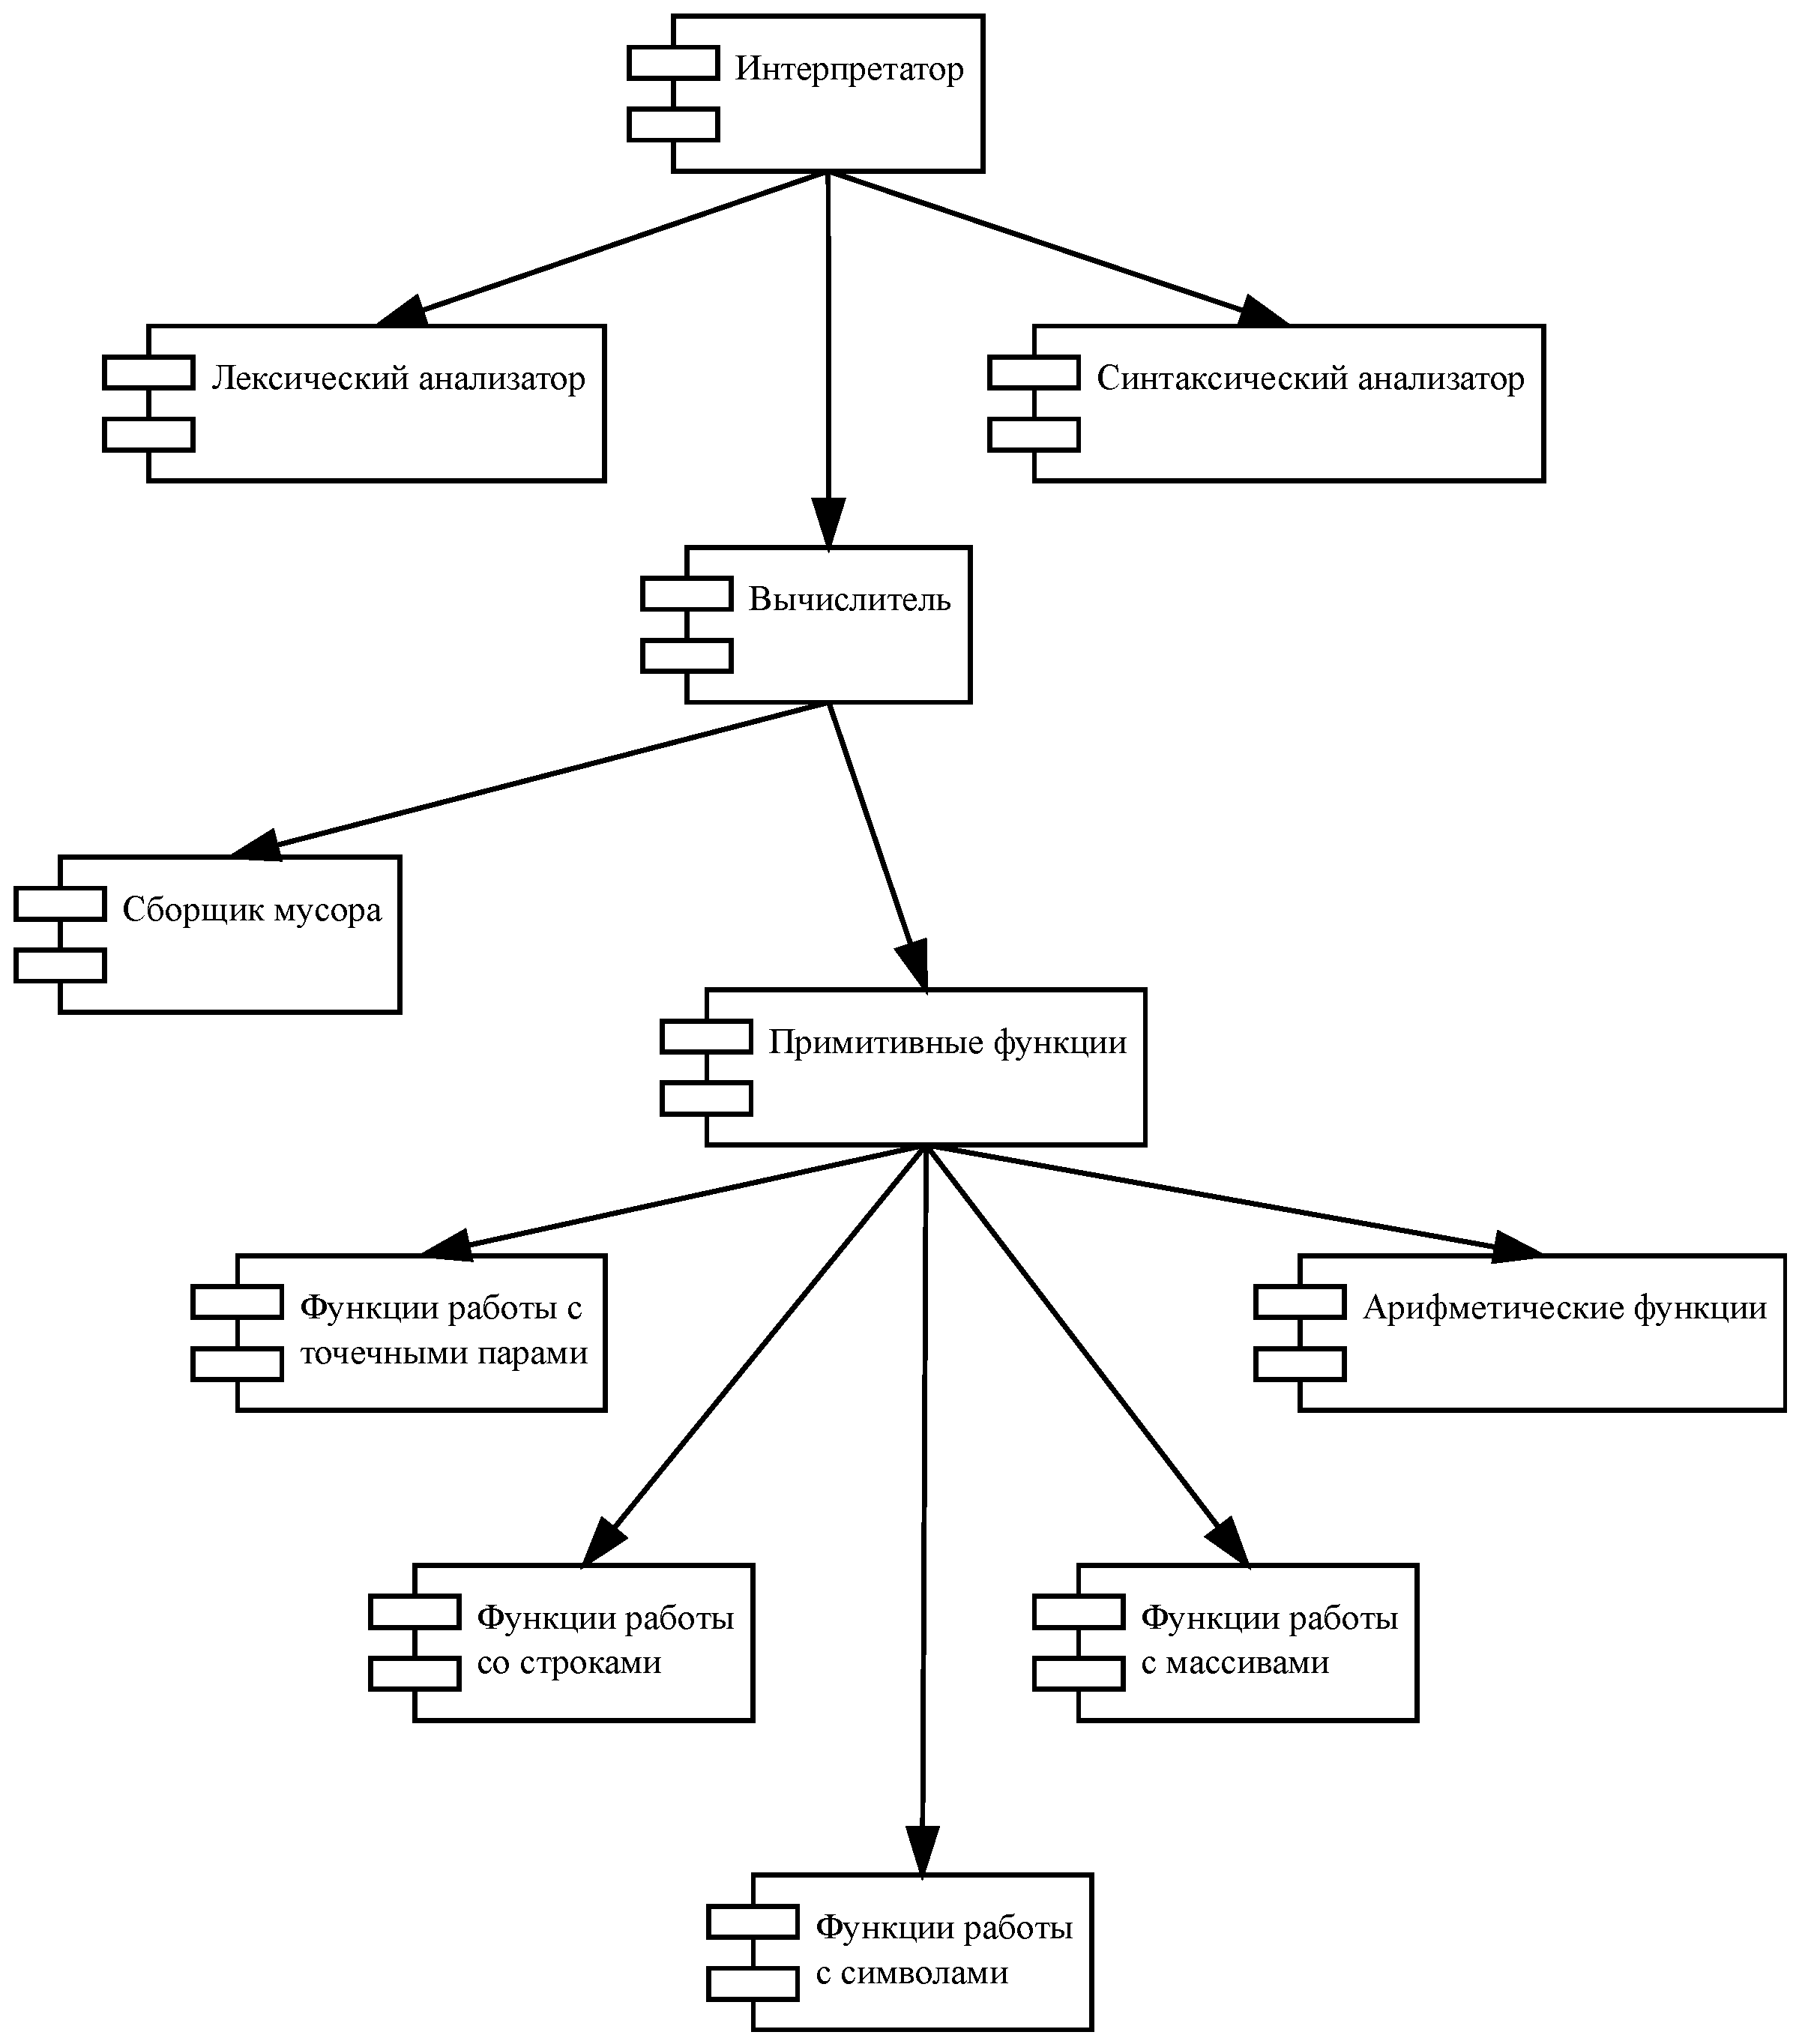
\includegraphics[width=1\linewidth]{kompdiagram}}
	\caption{Диаграмма компонентов интерпретатора}
	\label{kompdiagram:image}
\end{figure}

Таким образом, разработанный интерпретатор должен реализовывать следующие компоненты:
\begin{itemize}
	\item Лексический анализатор - для формирования токенов на основе текстового представления программы и выявления ошибок, связанных с использованием отсуствующих в алфавите языка символов или недопустимых в к использованию в некотором контексте символов (например, буква внутри числа: 124a6);
	\item Синтаксический анализатор - для формирования на основе токенов представления программы внутри интерпретатора и выявления синтаксических ошибок: отсутствие закрывающей скобки, отсутствие аргументов и тому подобные;
	\item Исполнитель - для выполнения инструкций, описанных в интерпретируемой программе;
	\item Сборщик мусора - для выявления и освобождения памяти, хранящей элементы, более не использующиеся интерпретатором;
	\item Примитивные функции - для реализации встроенных в язык функций, инструментов и конструкций, позволяющих производить манипуляции данными.
\end{itemize}


\subsection{Требования к программной системе}

\subsubsection{Требования к данным программной системы}
Программная система должна принимать на вход файл с кодировкой \quotes{UTF-8}, содержащий программный код на ДЯП.

\subsubsection{Требования к программному обеспечению}
Для реализации программной системы должны быть использованы: язык программирования \quotes{C}, реализация стандартной библиотеки языка - \quotes{glibc}.

Для сборки ПС требуется ОС семейства \quotes{GNU/Linux}, поддерживающая компилятор GCC версии \quotes{10.1} или новее.

\subsubsection{Требования к аппаратному обеспечению}
Для работы ПС необходим компьютер с архитектурой центрального процессора \quotes{x86} и свободной для использования пользовательскими процессами оперативной памятью от 64 Мб.

\subsection{Требования к оформлению документации}

Разработка программной документации и программного изделия должна производиться согласно ГОСТ 19.102-77 и ГОСТ 34.601-90. Единая система программной документации.
